\documentclass[11pt,a4paper]{article}
\usepackage{amsmath,amsfonts,amssymb,amsthm,epsfig,epstopdf,titling,url,graphicx,array}


\theoremstyle{plain}
\newtheorem{thm}{Theorem}%[]
\newtheorem{lem}[thm]{Lemma}
\newtheorem{fact}{Fact}%[chapter]
\newtheorem{assm}{Assumption}%[chapter]
\newtheorem*{assm*}{Assumption}
\newtheorem{prop}[thm]{Propositione}
\newtheorem*{cor}{Corollary}

\theoremstyle{definition}
\newtheorem{defn}{Definition}%[chapter]
\newtheorem{conj}{Conjecture}[section]
\newtheorem{exmp}{Example}[section]

\theoremstyle{remark}
\newtheorem*{rem}{Remark}
\newtheorem*{note}{Note}
\newtheorem*{prf}{Proof}



\title{Reformalizing Consensus}
\date{April 27, 2015}
\author{Vlad Zamfir \\
 			\\
 			\small With special thanks to Vitalik Buterin and Ethan Buchman}


\begin{document}

%Maybe put ccrg, ethereum logos on the title page?
\maketitle

\tableofcontents


\section{Abstract}

Traditional definitions of the consensus problem don't apply well to economic or blockchain-based consensus protocols, of which the first example of each is Satoshi Nakamoto's Bitcoin protocol. The coincidence of two independent inventions in consensus technology in one protocol, together with the absence of an already-present language for talking about these things has confused a lot of discourse about blockchain-based \emph{and} economic consensus. We will reformalize the question of consensus in a way that captures these technologies as well as those studied by ``traditional'' consensus research.

\vspace{0.5cm}


\section{Introduction}

\begin{defn}[Common Knowledge]
Information is \emph{common knowledge} between members of a group, if each of the members knows that each other member knows that information, and they all know that they all know that they know it, and so on ad infinitum.
\end{defn}

The consensus problem, traditionally, is understood to be the problem of defining protocols that computers on a network can use to update common knowledge in common knowledge. By this, traditional consensus research considers the consensus problem solved, in a given network environment and an upper bound on the number of crash or byzantine faults, if and only if computers on the network will be certain that any change they \emph{commit} to the \emph{consensus database} will also be commited by \emph{all correct nodes in a finite amount of time}. This is a sensible security definition, but Bitcoin doesn't explicitly guarantee that commitments are final, and the fact that byzantine faults are economically costly doesn't get captured, although it plays an important role in Bitcoin's stability. But before we treat blockchains and economic consensus, let us review the traditional consensus research.

\subsection{Traditional Consensus, an overview}

Traditionally, consensus protocols are tested by seeing if they can solve the consensus problem for one consensus state update, in a given network environment. Some number of clients, typically given as a proportion, are assumed to be complying with the protocol and are called ``correct'', while the rest of the clients are ``faulty'', which typically means one of two things:

\begin{defn}[Crash-fault]
A crash-fault is a failure to terminate a process, or a disconnection from the network.
\end{defn}

\begin{defn}[Byzantine fault]
A byzantine node can misbehave in an arbitrary way. 
\end{defn}

In a security analysis, byzantine nodes are typically assumed to be controlled by a single attacker, and crash-faults are considered to be a subset of byzantine faults.Additionally, we must rely on assumptions about the reliability of the network, and of the processors on the computers who maintain the consensus. We generally either assume that the network is synchronous or asynchronous: 

%should check this definition against literature
\begin{defn}[Synchronicity]
Network messages propagate and online processes terminate in a finite amount of time.
\end{defn}

\begin{defn}[Asynchronicity]
There is no finite upper bound on how much time a message can take to arrive at its destination, or on how long any process will take to terminate. 
\end{defn}

The basic idea is that the more synchronous a network, the more reliably you can distinguish a crash-fault from a slow process. Whereas in a more asynchronous network you can't reliably distinguish the faulty from the slow, at all. This makes an important difference in a protocol's ability to use \emph{timeouts} to coordate consensus. Checking whether timeouts are assumed to be synchronized between nodes is a good heuristic for checking if a protocol is \emph{unsafe} in asynchronous networks. 

The following result is educational, but isn't tailored to practitioners:

%should check this against literature
\begin{thm}[FLP Impossibility \cite{FLP}]
It's impossible to guarantee that consensus will be reached in a finite amount of time in an asynchronous network if an adversary can selectively cause one crash-fault at a time.
\end{thm}

This result should have been called ``the FLP unfortunately-only-almost-sure possibility result'' because in practice nodes are not able conspire to be selectively faulty at the opportune moments for an indefinite period of time. In practice, the FLP impossibility result does not pose a direct problem, because protocols will do multiple attempts in the event of a failure, and consensus is (almost) surely reached in a finite amount of time. Before we go to the next important result, let us define:

\begin{defn}[Consistency]
The property that every correct node has a copy of the same consensus database.
\end{defn}

\begin{defn}[Availability]
The consensus can process a change to the database in less than a finite amount of time.
\end{defn}

The research has focused on finding protocols that have consistency in asynchronous environments, even in the presense of byzantine faults. They regard the loss of consistency as a loss of common knowledge, and therefore a failure of consensus. The following result is relevant:

\begin{thm}[CAP Theorem \cite{CAP}]
If there is a network partition, then the consensus protocol must choose between availability and consistency.
\end{thm}

After establishing that a protocol can safely come to consensus (usually in an asynchronous model, while practitioners tend to deploy synchronous protocols), the traditional approach iterates this process in order to produce a changing consensus database that can be used by an application that has to be robust or available all the time. In practice, this turns out to be a difficult way to understand consensus.

This has led to growing interest in a strategy for teaching/learninc consensus, known as the \emph{replicated state machine approach} (Figure 1) that lends itself to being more easily understood by practitioners. Importantly for our context, it also makes it easy to bridge the gap between the definitions used to talk about traditional consensus protocols to a language that is useful for blockchain-based consensus protocols. The replicated state machine approach emphasizes how consensus protocols are used to append entries to the log which holds a record of a change to the state of the \emph{consensus application}, and it puts consensus into the context of client-server relationships, making it less abstract.

\begin{figure}
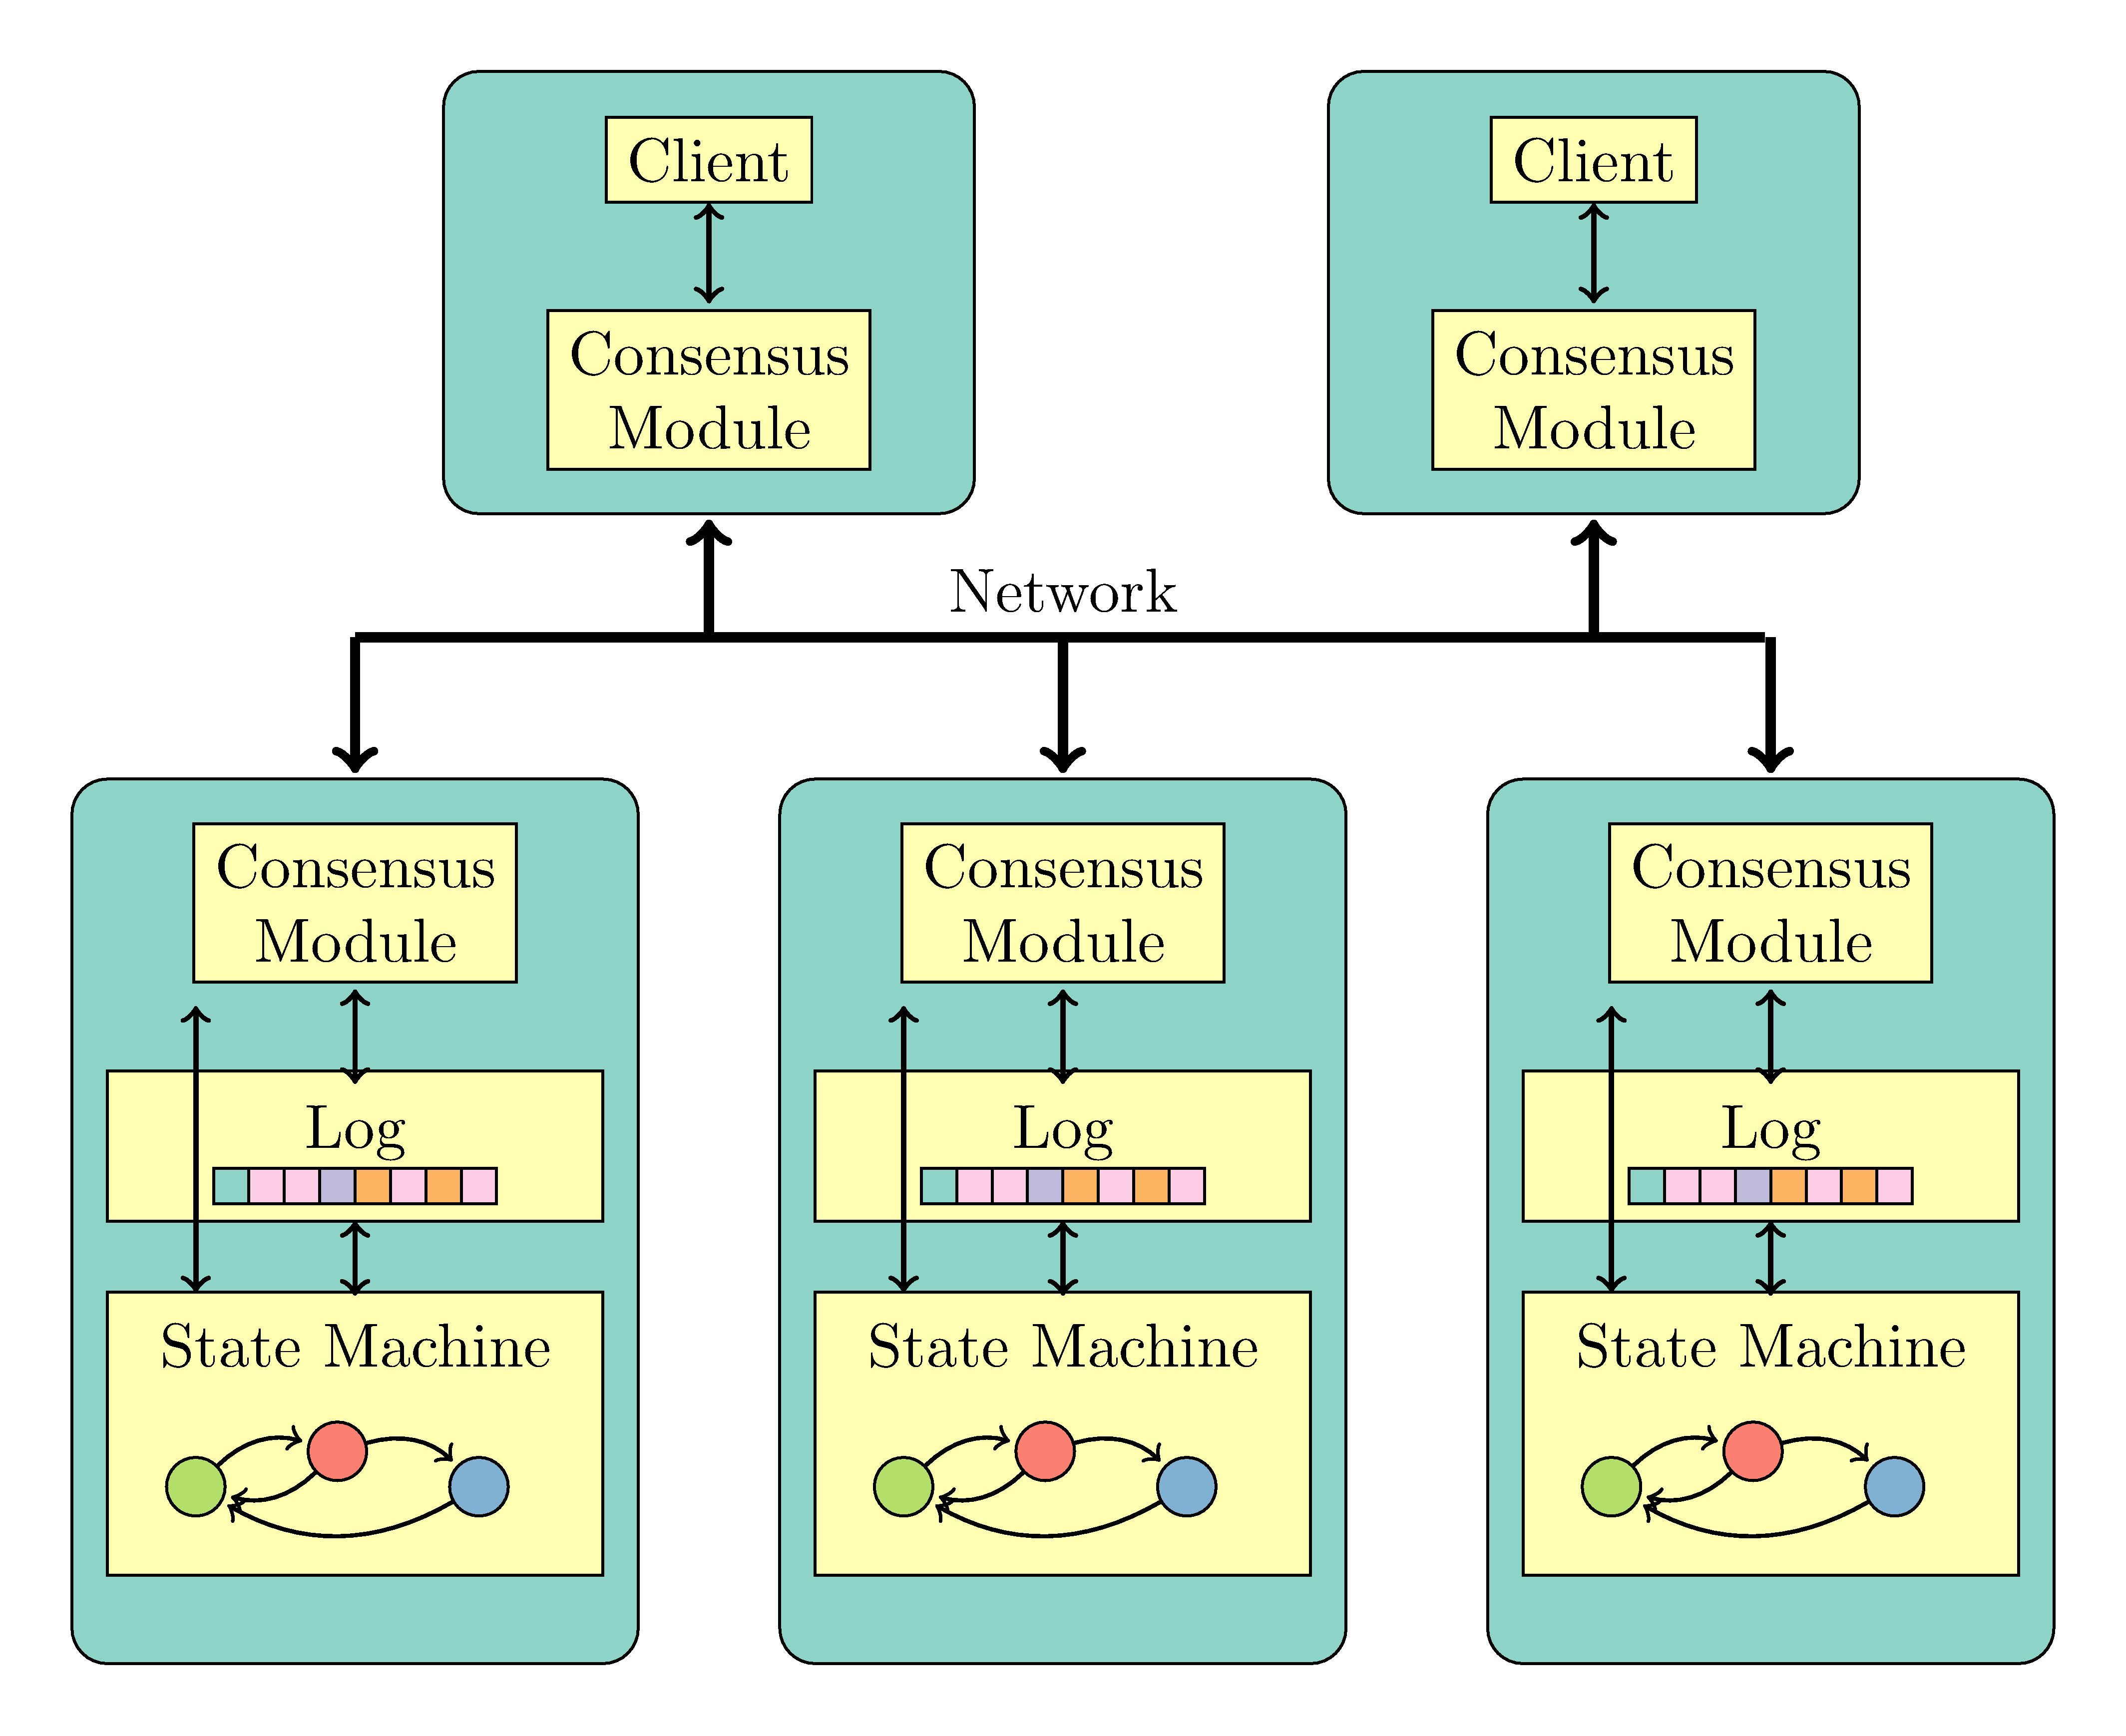
\includegraphics{smr.png}
\caption{A depiction of the replicated state machine approach, special thanks to Heidi Howard (@heidiann360) for the figure}
\end{figure}


\subsection{Bitcoin, the Blockchain, and Economic Consensus}

The Bitcoin consensus protocol can be understood in the replicated state machine approach as a consensus protocol that, instead of only adding to the replicated log, chooses between competing ``forks'' of the log. 
To be precise; this analogy isn't perfect because a block is not a log but a data structure that contains a group of logs, a cryptographic hash of ``the previous block'', along with some other information. The Bitcoin protocol requires that the hashes of the blocks be small enough, at considerable computational expense to the clients supporting the consensus by creating blocks, but it also issues digital assets to the ``miners'' who created these blocks. For miners to incur considerable computational expense, these assets must have a price, and they will only have a price if consensus is maintained by the miners. Additionally, clients choose the fork that has the most ``proof-of-work'' (a quantity of computational resources spent as infered from the hash value) and are able to maintain consensus because no adversary is willing or able to make a chain that is more computationally expensive to produce than the ``consensus fork'' \cite{Bitcoin}.

As you might see, this is both quite complicated and outside of the scope of traditional consensus research. Bitcoin gives economic guarantees that consensus will be maintained, and the only block on which clients have consensus, if we use traditional definitions, is the ``genesis block'', which is defined in the protocol as the first block. We are going to need new language and weaker definitions of the consensus problem to talk about blockchain-based or economic consensus protocols, in general, and it turns out that these are indeed independent inventions in consensus science. We will give an elementary language for talking about blockchains and economic consensus before we revisit Bitcoin and also conduct an analysis of Tendermint \cite{Tendermint}.

\section{Blockchain-based Consensus Protocols}

The main difference between a blockchain-based consensus protocol and a traditional consensus protocol is that clients in a blockchain-based protocol actively make choices between competing logs, while in a traditional protocol clients only append entries to their logs, and logs are mostly used to catch recovered clients up on missed changes to the consensus.
We will continue to assume that blocks are ordered logs together with other information, because this is in practice how blockchains work, even though for these definitions we could perhaps assume without loss of generality that blockchains are simply logs. 

\begin{defn}
A blockchain-based consensus protocol is a triple $(\mathcal{F}, \mathcal{S}, \Gamma)$, where:
\begin{itemize}
\item $\mathcal{F}$ is the fork-choice rule
\item $\mathcal{S}$ is the protocol-recommended consensus strategy
\item $\Gamma$ is the by-block application state transition function.
\end{itemize}
\end{defn}

The ``consensus strategy'' corresponds to the ``consensus module'' of Figure 1, and is so named because it represents the logic used by clients in an \emph{attempt} to come to consensus, and because it will coincide with language for economic consensus protocols. The protocol insists that $\Gamma$ is used to apply blocks to the state of the consensus applicatioin, and that clients use $\mathcal{F}$ to choose a blockchain. 

In order to make this a bit more formal, let us use $\mathcal{B}$ to denote all possible blocks, $\mathcal{C}$ to denote all possible blockchains, $\Sigma$ to denote all possible consensus application states, and $\mathcal{V}$ to denote the set of all possible \emph{client views}. Though we won't show here that we can do this without loss of generality, we will assume that $\mathcal{V} = \cup_{n \in \mathbb{N}}\left\{\mathbb{R} \times \mathcal{C}\right\}^n \cup \{\emptyset \}$, where the real number can be used to record the time at which the client first had a blockchain come into its view.

Then we can insist that:
\begin{itemize}
\item $\mathcal{F}:\mathcal{V} \to \mathcal{C} \cup \{\emptyset \}$
\item $\mathcal{S}:\mathcal{V} \to \mathcal{B} \cup \{\emptyset \}$
\item $\Gamma: \Sigma \times \mathcal{B} \to \Sigma \cup \{\emptyset \}$
\end{itemize}

Where the emptyset represent exceptions or waiting for processes to terminate or network events to occur.

Traditional consensus protocols are a subset of these blockchain-based consensus protocols, in the sense that they have a rule for changing the application state as a function of the logs, and a strategy for appending the logs to the consensus, while the fork-choice rule is trivial:

\begin{defn}[Trivial fork-choice]
A blockchain-based consensus protocol has a trivial fork-choice rule if clients never revert a log that has changed the state of their copy of the consensus application.
\end{defn}

We will also have an assumption that is a weaker version of the ``all correct nodes come to the same value'' assumption:

\begin{assm}
All clients use the fork-choice rule defined in the protocol to choose an application state for their copy of the attempted consensus.
\end{assm}

Before we define our attack model, let us give a couple of preliminary definitions:

\begin{defn}[Block]
A block is an ordered list of transactions (logs), together with a \emph{height} $h \in \mathbb{N}$, and a cryptographic hash of a block with height $h - 1$, and perhaps some additional information. 
\end{defn}

The definition is general enough, and it gives us the basic handles that we need to talk about blockchains:

\begin{defn}[A fork's tail]
A blockchain $f$'s \emph{tail at height $H$}, $f^H$, refers to the blockchain that has the same blocks for all heights $h \in [0,H]$, but no block at height $H + 1$.
\end{defn}

\begin{defn}[A blockchain's broom]
A blockchain $f$'s broom in a client's view $v \in \mathcal{V}$ is the set of all blockchains in $v$ who share only $f$ as a tail. Note that $f$ is called a handle, in this context.
\end{defn}

We can now define an attack on clients, to which only clients with a non-trivial fork-choice rule are vulnerable:

\begin{defn}[State reversion attack]
An attacker sends a client a broom with a handle that is shorter than the client's current fork-choice, with the intention or effect of causing the client to revert changes they made to the consensus state.
\end{defn}

We can additionally specify the height of the state reversion attack as the height of the attacking broom's handle. We also commonly call these attacks ``double-spend'' attack for historical, ``Bitcoin reasons'', but strictly speaking double-spending also involves adding something to the adopted fork that prevents another change to be commited to that fork. This more general attack is the most important attack against consensus protocols. We can use this by-client attack definition to give a security definition.

\begin{defn}[Pointwise Security]
The security of the tail $f^H$ of a client's fork choice $\mathcal{F}(v) = f$ is characterized entirely by the probability that that tail will no longer be a part of the client's blockchain of choice in the future, given a set of network and fault assumptions. 
\end{defn}

The question of whether or not consensus is guaranteed by a protocol is therefore is not simply a matter of how much asynchrony or faults of various kinds are required for the common knowledge to be lost, for the entire set of correct nodes - but a more complex question about how much asynchrony or faults are required for any particular subset of clients to abandon how much of their fork choices. This ``pointwise'' definition of security can be used to talk about how confident nodes can be that they share how much of a tail, given that they make a set of network and fault assumptions. 

In the traditional approach to consensus, we iteratively make non-repudiable changes to the consensus, so the problem is phrased in terms of maintaining common knowledge from step to step. In this broader class of consensus protocols, clients aim to grow the tails that their fork-choices have in common by abandoning what they might have thought was common knowledge when they see something more convincing. A security guarantee, therefore, might be something along the lines of ``unless more than a third of the clients are faulty, then in a synchronous network all correct clients will have a higher probability of having a longer common tail, in a finite amount of time''. Notice how this guarantee stresses the uncertainty that nodes can have about the state of the consensus, in this broader class of protocols.

It might, from the perspective of traditional consensus, seem that having a non-trivial fork-choice rule is unsafe - and they are correct, by their definition of safety. However, simultanously recall the CAP theorem and the fact that consensus systems are sometimes used because humans need to make sure that information services are always available. By focusing so much on a definition of safety in the context of ``one-off'' changes to common knowledge, consensus research has under-served systems that prefer availability to consistency in the event of faults or partitions. 

Blockchain-based consensus definitions of security, on the other hand, makes it clear to the practitioner that consensus is an iterative process of trial-and-error - as the ability to revert state changes to maintain consensus is invaluable in systems where availability is the first priority. It is our conclusion, therefore, that blockchain-based consensus is an innovation in consensus technology.


\section{Economic Consensus Protocols} 

Bitcoin was not only the first instance of a blockchain-based consensus algorithm, but it is also the first economic consensus protocol.

A consensus protocol is said to be economic if it makes byzantine faults expensive through the use of digital assets in the consensus state - a state that all nodes update according to rules defined by the protocol, $\Gamma$. This idea is a solution that can allow for the free entry and exit of nodes who maintain consensus - indeed, Bitcoin itself allows the ``miners'' who produce blocks to be anonymous. Very notably, Bitcoin mining has become an industry of businessmen who have spent and made hundreds of millions of dollars mining bitcoins. It is our position that this invention, rather than deft use of blockchain technology, is what has made Bitcoin a relative success.

This level of freedom to change the members of consensus group without a network administrator hasn't been treated as well by traditional consensus research because of the \emph{Sybil attack} problem, where an adversary can deliberately use the mechanism to increase the number of nodes in the group who are under their control over time. Economic consensus protocols make it expensive to be byzantine, and are therefore safe against Sybil attackers who are unwilling to budget and spend enough money. 

It is possible that non-compliant clients participate in the protocol's consensus in order to maximize their return in the protocol's digital asset. We will therefore modify our assumption that all non-byzantine clients are correct, as some clients will be profit-seeking, and especially as we can imagine that the consensus can be a public utility that anyone on the internet can serve or use. Instead of having only two possible compositions of nodes (correct, faulty) or (correct, byzantine), we will have a considerably more complex model, as some nodes will be economic actors. 

Practitioners who develop economic consensus protocols will likely have to be somewhat versed in economics, game theory, and mechanism design - as will the researcher who wants to analyze the security propositions of these protocols. Note that we will continue to use the notation defined in the section on blockchain-based consensus.

\begin{defn}[Rational]
A client is said to be rational if they will change their consensus strategy $\mathcal{S}$ if it makes or saves them money.
\end{defn}

\begin{defn}[Compliant]
We will now refer to ``correct'' nodes as \emph{compliant}, avoiding the implication that it's incorrect to be rational.
\end{defn}

We will use what we believe is a worst-case attack model, for how an attacker with a budget can influence the behaviour of rational nodes:

\begin{defn}[Bribe attack]
An incentive attack where the attacker commits money to an incentive mechanism which promises to pay clients under some circumstances, with the intention or effect of causing rational nodes to change their consensus strategies. We additionally assume that: 
\begin{itemize}
\item the attack has no coordination costs
\item rational nodes immediately become aware of bribes
\item rational nodes are able to efficiently calculate whether a change in software will increase their profitability.
\end{itemize}
\end{defn}

Motivated by the fact that it doesn't seem right that only the rational nodes can change their consensus strategy, and by our previous definition of byzantine nodes, we define alturist nodes as anti-byzantine nodes:

\begin{defn}[Alturist]
An altruistic node are able to change their code in an arbitrary way, even at their own expense, but in a security analysis are assumed to work against the attacker.
\end{defn}

A canonical security analysis, therefore, will aim to give or test the security guarantees of an economic consensus protocol given the assumption that $b$ nodes are byzantine (and do not need to be bribed by the attacker, at all), $a$ nodes are altruist, $r$ nodes are rational, $c$ nodes are compliant, as well as a bribing attacker's budget $b$ along with the traditional networking assumption. This is certainly more complicated than the typical analysis of a consensus protocol, because the results of economic analysis are often dubious, but it captures the worst-case analysis, given a particular attack budget, and is therefore more satisfactory than traditional byzantine fault tolerance analysis, which does not let you assign a dollar-valued cost to these faults. 

If secure economic consensus protocols are possible, then they may have the potential to provide services that were previously impossible. For example, economic consensus could be used to create a sustainable public internet-based-utilities that can be used as a public source of authenticated, always-available information services - in a system that can outlast human organizations who would otherwise be trusted to provide the services, or even resist attack by a powerful adversary. Economic consensus also promises to allow companies and governments who do not trust each other to share a common application state that they can trust without common knowledge that they are all following the protocol-recommended consensus strategy. These and other possibilities will push practitioners and researchers alike to continue work on the topic, even though the legal status and technical viability of distributed economic consensus protocols is questionable.

The biggest problem for economic consensus protocol design for the public internet is perhaps that if economic clout isn't distributed evenly in the economy outside of the consensus, then it will also tend to be centralized in the consensus, so long as the inability to spend money is the only thing prohibiting nodes from becoming part of the consensus group. This means that we won't generally be able to assume that there is perfect competition between clients, so instead we should assume that consensus nodes form profit-maximizing coalitions.

Finally, we should note that non-economic consensus protocols are a subset of economic consensus protocols; assuming that the digital assets defined in the consensus has a price of zero, the analysis collapses back to a more ordinary byzantine fault tolerance analysis, where rational nodes are byzantine. Now, we will conduct analysis of the Bitcoin consensus protocol, and then of the Tendermint consensus protocol - both of which are economic blockchain-based consensus protocols - to demonstrate the language shared here.



\section{Analysis of Bitcoin}

Let us denote Bitcoin's consensus protocol as $\mathcal{P} = (\mathcal{F}, \mathcal{S}, \Gamma)$, for convenience and consistency. 

Bitcoin's fork-choice rule $\mathcal{F}$ is to choose the fork with the most proof-of-work. The protocol-suggested consensus strategy $\mathcal{S}$ is to produce blocks at the head of $\mathcal{F}$'s choice. Finally, the state transition function $\Gamma$ processes transactions and rewards an address that the miner placed in the block, with Bitcoin issuance and transaction fees. Bitcoin is a very simple and elegant blockchain-based economic consensus algorithm, in terms of its specification, but the security analysis is not trivial.

Bitcoin manages asynchrony in an interesting way: instead of using timeouts, it assumes an upper bound on the computational capacity on the network of computers that mine blocks, and targets the difficulty of a brute-force computational puzzle so that blocks are produced at an average rate of 10 minutes. The fact that creating proof-of-work is a low-probability event that cannot be spoofed, but isn't a digital signature, allows Bitcoin to be an effectively-leaderless anonymous consensus protocol, where miners only need to broadcast to each other the blocks that they find, not needing to know each other's locations or latencies. While it may at first glance make it seem like Bitcoin is asynchronous, we will see that Bitcoin's security guarantees rely on a synchronous network between miners. However, it is good to see how Bitcoin works in optimistic scenarios, like in a synchronous networks with compliant nodes:

When a miner finds a block, they publish it to the rest of the miners, who stop mining on the old head of the chain, and now mine on the block they just received. This keeps the Bitcoin blockchain growing in one direction, rather than forking. There are occationally \emph{orphaned blocks}, when two miners find blocks at the same height at around the same time, and hence could not coordinate to stack the blocks. Technically these orphan blocks could stack up into longer forks, but the probability of creating orphan blocks is low and the probability of ``simultanously'' finding blocks declines exponentially in the number of blocks and a time, and in the number of times, so miners are in practice able to coordinate on one fork.

The fact that Bitcoin has a price and is being issued to the network for doing proof of work, assuming that mining is an efficient market, means that an attacker would have to pay a bit more than the issuance-plus-fees given to miners, in order to produce blocks with more work than the consensus. At the time of writing the price of Bitcoin is 228 USD, with 25 Bitcoins issued per block every 10 minutes, for 24 hours a day means that Bitcoin is spending an astonishing 820,800 USD per day. In return, an attacker would have to spend more than that, to create a one-day fork, assuming the network is synchronous and all nodes are compliant.

This high price of security of consensus is one of the primary arguments against using Bitcoin's consensus protocol. The common counterargument is that this is a distribution mechanism that builds a useful network effect, and the protocol does define that issuance halves every four years. Many feel, however, that Bitcoin will become insecure if or when the level of issuance falls according to schedule.

Now, let us see what happens to Bitcoin in asynchronous conditions. In the event of a network partition, with half of the mining power on one side and the other half on the other, it will be half as hard for an attacker to produce more proof-of-work in a single chain than the network. Therefore, Bitcoin's security relies on a sufficienly frequently connected network, something that can't be guaranteed in asynchronous network models. Therefore, even though Bitcoin is technically available during a partition, its security guarantees are not as available. Worst of all, it is unable to give clients a prompt indication that their guarantees have weakened; they must wait to observe that blocks which occured at random times are now occuring less frequently due to the partition or find extra-consensus sources of the information.

Now, let us assume once more than the network is synchronous, but we will assume that all of the nodes are rational. The immediate concern, now, is that the timestamps that Bitcoin uses in order to coordinate the difficulty of creating blocks so that blocks come at a predictable rate are not reliable, as the protocol has no way to punish nodes if they lie about the timestamp, which they would happily do in return for a bribe of $\epsilon$. A reader with traditional inclinations might object to the use of rationality instead of compliance to the protocol, in a security analysis, but the existence of rational deviations from the protocol-suggested strategy exist in practice. 

Bitcoin mining pools are a canonical example of how clients will change their software in order to make more, or, in this example, more steady returns. Mining pools are lottery pools for discovering blocks; these pools are necessary for clients with a small amount of mining power to reduce the volatility of their Bitcoin returns for mining. They are not a part of the consensus protocol, but in practice they are an important part of Bitcoin's infrastructure today. Rational changes to the consensus strategies of nodes is not necessarily bad, but it does and will continue to happen, and therefore constitutes an important security consideration. Let us therefore continue down the rabbit hole of assuming that Bitcoin's miners are rational.

If we assume that mining pool operators are rational, and that they make more returns for having a larger share of the global mining power, then the mining pools are involved in an adversarial game. It is important that all blocks propagate to all miners quickly, for things to be fair, because Bitcoin miners mine on the head of the chain until they see a new block. A ``selfish miner'' will be able to get a marginal advantage, if they have sufficient mining power, by delaying the publication of his block, so he has a head start mining at the next height, at only a small chance that his block will be orphaned due to his delay. Rational mining pools will engage in selfish mining, and this will increase the returns of their miners. \cite{SelfishMining}

Moreover, there is another, much more insidious attack. A mining pool can sign some of their mining power up with another pool - claiming returns for proving that they are doing work, but withholding blocks from that pool, when they are found. The effect is that the mining pool that is having blocks withheld from it will be paying out revenues to miners who aren't contributing to the pool, while the attacking pool is giving up only a small amount of revenue by withholding the block, giving the attacking pool a competitive advantage but making the miners of both pools worse off. In the scenario where this strategy is common, mining pools need to assign and redundantly search areas of nonce-space in order to catch miners who are withholding blocks. The equilibrium of this situation might be that every pool checks every nonce twice, but showing that is outside the scope of this analysis. \cite{BlockWithholding}

Lastly, the \emph{P + $\epsilon$} attack is the most damning attack on the Bitcoin protocol, as it succeeds in perfectly synchronous networks assuming that more than half of the miners are rational, and, remarkably, without spending any of the attacker's budget. The attacker tells the miners to mine on his attacking fork, and that if the attack fails that the attacker will pay them more than the mining reward they would have earned mining on the ``consensus fork''; however, if the attacker's fork wins, the protocol pays the miners who participated in the attack, but not the miners who mined on the victim fork. Therefore, it is a strictly dominant strategy for the miners to participate in the attack, and the attacker spends none of his budget. \cite{P_Plus_Epsilon}

Now that we know that the attacker can control rational nodes for free, in our model, we are ready to state Bitcoin's security guarantee:

Recalling that $b$ denotes the proportion of miners that is byzantine, $a$ the proportion that is alturistic, $r$ the proportion of rational nodes, and $c$ the remaining proportion of nodes who are compliant, and now also denoting Bitcoin miners' reward per block as $R$, and assuming that mining is an efficient market and that the network's largest partition has $h\%$ of the overall hashing power, then we can say that an attacker must spend $h \cdot R \cdot max\{(a + c) - (b + r),0\}$ per block of the attacking fork. This security guarantee is much weaker than what most people suppose that Bitcoin guarantees, and is in our opinion much less than it deserves for the price tag. 

It might be that in practice, extra-protocol phenomena, attack coordination costs (which were assumed to be zero), or plain lack of interest mean that Bitcoin will survive any attention it gets from adversaries. Alternatively, it might get out-competed on a market between economic consensus protocols, and will be forced to coordinate a change to its consensus protocol by popular demand rather than due to repeated attack. 

\pagebreak
\section{Analysis of Tendermint}

Let us reuse notation and denote the Tendermint protocol as $\mathcal{P} = (\mathcal{F}, \mathcal{S}, \Gamma)$. 

Tendermint is a security-deposit-based, economic consensus protocol invented by Jae Kwon\cite{Tendermint}. It has a consensus strategy $\mathcal{S}$ that is based on a traditional byzantine fault tolerant consensus algorithm. It uses a 3-phase commit protocol that is guaranteed to terminate in the presence of up to 33\% byzantine faults in a partially synchronous networks (i.e. asynchronous for unbounded but finite intervals of time), that the \emph{bonded validators} use to coordinate a decision on exactly one block at every height. The commit represents both a commitment to never revert the corresponding change to the consensus database, and a guarantee against byzantine faults because producing commits for more than one block at the same height is punishable by forfeiture of their security deposit - this is a policy enforced by $\Gamma$, which is executed by every validator to update the consensus state. Tendermint therefore has a trivial fork choice rule - online clients never revert changes that are commited. Offline clients that catch up to find that there is more than one fork with 67\% of validators return an exception, because they were expecting that only up to 33\% of validators would be faulty, but 34\% of the validators had to double-commit to create a fork.

Tendermint is technically somewhat more complicated than Bitcoin's protocol, but the security analysis is much easier, and it will be more familiar to readers with a background in traditional consensus. Let us conduct the analysis in the same order as we did with Bitcoin, first examining how it works when all nodes are compliant and the network is synchronous:

Assuming that clients currently have consensus, the protocol guarantees that they will have consensus on an order in which the bonded validators are to propose blocks so that the validators can attempt to commit to that block. Because the network is synchronous, the validators will be able to agree on whose turn it is to propose a block, and will be able to publish and observe 67\% of the validation ``pre-vote'' signatures, then on the condition that they have these pre-vote signature stored they publish a ``pre-commit'' signature. Once any client has 67\% of the validator ``pre-commits'', all nodes are expected to commit to the block. However, Tendermint nonetheless requires that the number of byzantine nodes be no greater than than 33\%, because an inability to get 67\% of validation signatures on any stage will make the validators unable to commit further changes. 

Before we do the security analysis for the optimistic synchronous compliant model, let us do the analysis for all-rational nodes as it is a bit simpler. The first thing to notice is that if all bonded validator nodes are rational, then the attacker would have to pay $\epsilon$ more than 34\% of the issuance and fees that validators earn per minute in order to halt the consensus. This is not necessarily very bad, but it is certainly worth noting. The next thing is that the creation of a valid fork would cost an attacker $\epsilon$ more than 34\% of the total amount on security deposit, as this is the minimum amount of double-signing that occurs when a fork is created. This is in stark contrast with the zero-cost attack on Bitcoin that is possible if all miners are rational; that mining power is an external resource, while a security deposit can be removd by the protocol itself, upon detection of a byzantine fault.

To create a fork in Tendermint if all nodes are compliant and the network is synchronous, you would have to bond more than twice the amount of stake on deposit, in order to have 67\% of the bonds to sign the 2nd block at the height of the fork. Then you would lose 34\% of the bonds at that time, which is approximately equal to the amount of stake currently on deposit. Therefore, it costs around 100\% of the currently bonded stake to create a fork in Tendermint, if all clients are compliant and the network is synchronous. If clients are compliant and the network is partially synchronous (asynchronous for finite amounts of time), it will be possible for the attacker to bond only a bit more than 100\% of the deposits and fool asynchronized disjoint but compliant sets of validators into signing two different blocks at the same height, and then would lose the standard 34\% of bonds - which corresponds to 67\% of the initial total bonded stake. 

It is very notable that when the network is asynchronous, Tendermint is unable to coordinate on when it is a client's turn to propose a block, and consensus is halted. This is perhaps unfortunate because there exist byzantine fault tolerant algorithms for electing leaders in asynchronous networks. It may eventually be worth the additional complexity for Tendermint to also provide almost-sure guarantees of finality in an asynchronous network with no more than 33\% byzantine faults.

The economic security analysis of Tendermint, so far, has given very optimistic results. Certainly more than a third of the stake currently on deposit will be lost by byzantine nodes when a fork occurs. This high cost combined with the strong preference for consistency over availability makes Tendermint an attractive alternative to Bitcoin, in particular if a significant proportion of Bitcoin nodes are rational. However, an analysis of the stability of coalitions between rational bonded validators, credited to Matthew Wampler-Doty, gives a more pessimistic outlook:

If a coalition of at least 67\% of the validators forms, they can exclude the rest of the validators from having their blocks commited or their signatures included, thereby increasing their share of transaction fees and becoming more profitable. After these excluded validators are unbonded, we will once again have the same situation, where a coalition of 67\% or more of the now-still-bonded validators can profit by excluding the validators in a minority. This analysis has two possible equilibriums: either the two initially most powerful validators to remain, each having at least 34\% of the bonds so that they cannot be removed by the other, or only the initially most powerful validator remains in the validator set. 

The common refutation to this line of argument is that the validators will be forced to cooperate because their users will use another consensus if Tendermint is perceived to be centralized. This argument relies on the inability of the coalitions to keep their byzantine behaviour secret or accepted - something that might be true in practice - but we would prefer to have rational behaviour be driven by in-protocol incentives as much as possible, in security analysis, and are not satisfied that there is nothing more to be done to prevent hostile majority coalitions from forming. It is therefore unclear if the equilibrium of Tendermint validation is sufficiently decentralized to form the basis of a public utility.

The last notable concern for some applications is that Tendermint, by choosing a trivial fork-choice rule and a traditional consensus protocol as its consensus strategy, is forced to choose consistency over availability in the face of network asynchrony or partitions. While this may be appropriate for Tendermint's intended use-cases, it may not be suitable for applications that must be available, above all else. 


\section{Conclusion}

Both blockchains and economic consensus protocols are non-trivial to design and analyze. The goal of this work has been to share a language that we can use to talk more formally about these things without conflating or confusing them. It should be clear that much work remains to be done: 

Blockchain technology promises to help us build consensus protocols that are available in asynchronous networks, but most research into blockchain technology to date has focused predominantly on economic consensus.

Economic consensus protocols promise to create backbones for public utilities, but it isn't yet clear that there exists an economic consensus protocol that is suitable for the role in an environment where all nodes are rational and wealth is not uniformly distributed.

\pagebreak

\bibliographystyle{plain}
\bibliography{mybib}

\end{document}